\clearpage
\thispagestyle{empty}
\null
\newpage

\cleardoublepage
\phantomsection
% \pdfbookmark[1]{Etat de l'art}{Etat de l'art}
% \addcontentsline{toc}{part}{Etat de l'art}
\markboth{\spacedlowsmallcaps{Etat de l'art}}{\spacedlowsmallcaps{Etat de l'art}}
\part{Etat de l'art}
\label{part:etat_art}

\clearpage
\thispagestyle{empty}
\null
\newpage

\chapter*{Introduction}
\addcontentsline{toc}{chapter}{\textbf{Introduction}}

\noindent
Cette seconde partie du manuscrit constitue un socle fondamental pour la compréhension de notre démarche. Elle expose les cadres théoriques et concepts mobilisés, tout en identifiant les verrous scientifiques qui motivent les hypothèses formulées en \autoref{part:contexte} et la méthode proposée par la suite.

Elle poursuit un double objectif. D'une part, introduire les notions clés issues de la littérature sur les \acn{SMA}, les modèles organisationnels, le \acn{MARL}, et la modélisation d'environnements par apprentissage (World Models). Ces briques conceptuelles structurent notre approche de conception et doivent être clarifiées, articulées, et situées par rapport à leurs limites actuelles, notamment dans un contexte comme celui de la cyberdéfense.

D'autre part, cette partie met en relation les différentes hypothèses (H1 à H4) avec les lacunes de l'état de l'art, en identifiant pour chacune un verrou théorique ou technologique. Cette analyse permet de justifier l'originalité et la pertinence de notre méthode, en montrant que les approches existantes ne permettent pas de couvrir, à elles seules, les exigences du problème posé. Pour cela, le \autoref{chap:concepts} présente d'abord les principales briques théoriques de notre travail~: la structuration organisationnelle des \acn{SMA} via $\mathcal{M}OISE^+$, les principes et défis du \acn{MARL}, et les approches de simulation basées sur les World Models. Le \autoref{chap:verrous} approfondit ensuite les verrous associés aux hypothèses H1 à H4, en identifiant les manques de la littérature actuelle face aux objectifs que nous poursuivons.

La figure ci-après synthétise l'organisation de cette partie et les liens logiques entre les chapitres, sous-sections et objectifs.


\begin{figure}[h!]
  \centering
  \resizebox{\textwidth}{!}{%
    \begin{tikzpicture}[
    chapter/.style={draw, fill=blue!10, thick, minimum width=8cm, minimum height=1.2cm, text centered, font=\bfseries},
    section/.style={draw, fill=blue!5, thick, minimum width=7cm, minimum height=1cm, text centered, font=\small},
    arrow/.style={-Latex, thick},
    node distance=0.4cm,
    annotated/.style={above,font=\small\itshape, inner sep=1pt, yshift=0.8cm, xshift=-7cm}
]

% Chapitre 4
\node[chapter] (ch4) {\parbox{10cm}{Chapitre 4 : Les SMA et concepts théoriques mobilisés}};

\node[section, below=1cm of ch4, xshift=-1cm] (ch4s1) {\parbox{8cm}{SMA et modèles organisationnels}};
\node[section, below=1cm of ch4s1] (ch4s2) {\parbox{8cm}{Apprentissage par renforcement multi-agent}};
\node[section, below=1cm of ch4s2] (ch4s3) {\parbox{8cm}{Modéliser un environnement simulé : les techniques \textquote{World Models}}};

\draw[arrow] ($ (ch4.south) + (4.0,0) $) -- ++(0,0) |- (ch4s1.east) node[annotated] {Les bases du raisonnement organisationnel sont introduites pour structurer le comportement des SMA.};
\draw[arrow] ($ (ch4.south) + (4.0,0) $) -- ++(0,0) |- (ch4s2.east) node[annotated] {Ce cadre organisationnel doit être articulé avec les techniques d’apprentissage multi-agent.};
\draw[arrow] ($ (ch4.south) + (4.0,0) $) -- ++(0,0) |- (ch4s3.east) node[annotated] {L’apprentissage nécessite un environnement simulé, souvent construit par des World Models.};


% Chapitre 5
\node[chapter, below=1cm of ch4s3, xshift=1cm] (ch5) {\parbox{10cm}{Chapitre 5 : Revue de littérature, analyse et verrous liés aux hypothèses}};

\node[section, below=1cm of ch5, xshift=-1cm] (ch5s1) {\parbox{8cm}{Un cadre Markovien pour formaliser le problème \\ de conception et sa résolution en MARL (H1)}};
\node[section, below=1cm of ch5s1] (ch5s2) {\parbox{8cm}{Les Worlds Models pour simuler des \\ environnement multi-agents (H2)}};
\node[section, below=1cm of ch5s2] (ch5s3) {\parbox{8cm}{L'intégration de contraintes/guidages \\ organisationnelles dans le processus MARL (H3)}};
\node[section, below=1cm of ch5s3] (ch5s4) {\parbox{8cm}{L'extraction automatisée des spécifications \\ organisationnelles émergentes (H4)}};

\draw[arrow] ($ (ch4.south) + (4.5,0) $) -- ($ (ch5.north) + (4.5,0) $) node[annotated, yshift=-0.5cm] {À partir de ces concepts, chaque hypothèse est examinée à travers une revue ciblée.};

\draw[arrow] ($ (ch5.south) + (4.0,0) $) -- ++(0,0) |- (ch5s1.east) node[annotated] {La première étape consiste à formuler formellement le problème de conception.};
\draw[arrow] ($ (ch5.south) + (4.0,0) $) -- ++(0,0) |- (ch5s2.east) node[annotated] {Cela suppose la disponibilité d’un environnement simulé fidèle aux dynamiques réelles.};
\draw[arrow] ($ (ch5.south) + (4.0,0) $) -- ++(0,0) |- (ch5s3.east) node[annotated] {Dans ce cadre simulé, l’apprentissage doit être guidé par des contraintes organisationnelles.};
\draw[arrow] ($ (ch5.south) + (4.0,0) $) -- ++(0,0) |- (ch5s4.east) node[annotated] {Enfin, les comportements appris doivent pouvoir être interprétés sous forme de structures émergentes.};

\end{tikzpicture}

  }
  \caption{Structure de la Partie II~: Etat de l'art}
  \label{fig:organisation_manuscrit_partie_2}
\end{figure}

\clearpage
\thispagestyle{empty}
\null
\newpage

\chapter{Les concepts théoriques mobilisés}
\label{chap:concepts}

\noindent
Ce chapitre introduit les fondements théoriques sur lesquels repose notre approche de conception automatisée de systèmes multi-agents guidés par apprentissage. Il clarifie les concepts mobilisés, leurs articulations, ainsi que les limites actuelles de leur combinaison.

En particulier, trois sujets fondamentaux sont au cœur de nos contriobjectifions~:
\begin{itemize}
  \item les \textbf{modèles organisationnels} qui apportent une structure explicite pour organiser, coordonner et contraindre les comportements~;
  \item le \acn{MARL}, qui permet aux agents d'adapter leurs politiques à partir de l'expérience, dans des contextes potentiellement partiellement observables.
  \item les \textit{World Models}, qui permet de capturer la dynamique des transition d'observation, permettant indirectement de simuler l'environnement.
\end{itemize}

Dans ce chapitre, nous présentons successivement les modèles organisationnelle pour les \acn{SMA}, les principes du \acn{MARL}, puis les approches de modélisation d'environnement utilisées pour la simulation dont les \textit{World Models}.


\section{SMA et modèles organisationnels}

\subsection{Des SMAs aux modèles organisationnels}

Comme dit précédemment, un \acn{SMA} désigne un ensemble d'agents autonomes interagissant au sein d'un environnement commun afin d'atteindre des objectifs individuels et/ou collectifs. Chaque agent est défini comme une entité capable de percevoir partiellement son environnement, d'agir selon ses propres objectifs et d'interagir avec d'autres agents à travers des modes de coordination explicites ou implicites. Les \acn{SMA} se distinguent par plusieurs caractéristiques clés : autonomie locale (décisions sans supervision centralisée), hétérogénéité (diversité des capacités, objectifs ou connaissances), interaction sociale (collaboration, négociation, gestion des conflits) et émergence (propriétés globales issues de comportements locaux coordonnés).

Ces caractéristiques soulignent que les SMA sont particulièrement adaptés aux environnements distribués, dynamiques ou incertains, où la centralisation devient inefficace voire impossible. Toutefois, dans de nombreux cas, les interactions entre agents sont trop complexes ou critiques pour être laissées à une coordination purement implicite ou émergente. Il devient alors nécessaire d’introduire une organisation explicite afin de structurer le système, définir les responsabilités, réguler les interactions et guider l’activité collective.

L’introduction d’un modèle organisationnel permet d’assurer une cohérence globale entre les actions individuelles, de faciliter la réutilisation et la scalabilité des systèmes, d’améliorer la contrôlabilité et l’explicabilité des décisions collectives, ainsi que de spécifier des contraintes normatives sur le comportement des agents.

\subsection{Le modèle organisationnel $\mathcal{M}OISE^+$}

\begin{figure}[h!]
  \centering
  


\tikzset{every picture/.style={line width=0.75pt}} %set default line width to 0.75pt        

\begin{tikzpicture}[x=0.75pt,y=0.75pt,yscale=-1,xscale=1]
%uncomment if require: \path (0,1656); %set diagram left start at 0, and has height of 1656

%Shape: Rectangle [id:dp6756844921493015] 
\draw  [fill={rgb, 255:red, 248; green, 231; blue, 28 }  ,fill opacity=1 ] (46,1204) -- (214,1204) -- (214,1424) -- (46,1424) -- cycle ;
%Shape: Rectangle [id:dp3759944257810566] 
\draw  [fill={rgb, 255:red, 80; green, 227; blue, 194 }  ,fill opacity=1 ] (390,1204) -- (556,1204) -- (556,1424) -- (390,1424) -- cycle ;
%Shape: Rectangle [id:dp28244406216006945] 
\draw  [fill={rgb, 255:red, 144; green, 19; blue, 254 }  ,fill opacity=1 ] (218,1234) -- (386,1234) -- (386,1338) -- (218,1338) -- cycle ;
%Shape: Rectangle [id:dp32232123359581766] 
\draw   (42,1176) -- (562,1176) -- (562,1428) -- (42,1428) -- cycle ;
%Shape: Rectangle [id:dp7605706269262755] 
\draw  [fill={rgb, 255:red, 74; green, 144; blue, 226 }  ,fill opacity=1 ] (396,1286) -- (550,1286) -- (550,1418) -- (396,1418) -- cycle ;
%Shape: Rectangle [id:dp33110985390647496] 
\draw   (52,1294) -- (210,1294) -- (210,1418) -- (52,1418) -- cycle ;
%Shape: Rectangle [id:dp8653560038381976] 
\draw  [fill={rgb, 255:red, 245; green, 166; blue, 35 }  ,fill opacity=1 ] (52,1294) -- (210,1294) -- (210,1418) -- (52,1418) -- cycle ;
%Straight Lines [id:da09781093164567278] 
\draw    (412,1350) -- (353.61,1307.18) ;
\draw [shift={(352,1306)}, rotate = 36.25] [color={rgb, 255:red, 0; green, 0; blue, 0 }  ][line width=0.75]    (10.93,-3.29) .. controls (6.95,-1.4) and (3.31,-0.3) .. (0,0) .. controls (3.31,0.3) and (6.95,1.4) .. (10.93,3.29)   ;
%Straight Lines [id:da3938396723807833] 
\draw    (122,1334) -- (264.04,1304.41) ;
\draw [shift={(266,1304)}, rotate = 168.23] [color={rgb, 255:red, 0; green, 0; blue, 0 }  ][line width=0.75]    (10.93,-3.29) .. controls (6.95,-1.4) and (3.31,-0.3) .. (0,0) .. controls (3.31,0.3) and (6.95,1.4) .. (10.93,3.29)   ;
%Shape: Rectangle [id:dp269311335478327] 
\draw  [color={rgb, 255:red, 208; green, 2; blue, 27 }  ,draw opacity=1 ][line width=1.5]  (66,1322) -- (122,1322) -- (122,1334) -- (66,1334) -- cycle ;
%Shape: Rectangle [id:dp7449860119164387] 
\draw  [color={rgb, 255:red, 208; green, 2; blue, 27 }  ,draw opacity=1 ][line width=1.5]  (412,1342) -- (488,1342) -- (488,1354) -- (412,1354) -- cycle ;


% Text Node
\draw (472.5,1237.41) node   [align=left] {\begin{minipage}[lt]{112.2pt}\setlength\topsep{0pt}
\begin{center}
\textbf{{\small Functional Specs.}}
\end{center}
{\small  - Social schemes $\displaystyle \mathcal{SCH}$}\\{\small  - Social preferences $\displaystyle \mathcal{SP}$}
\end{minipage}};
% Text Node
\draw (474,1355) node   [align=left] {\begin{minipage}[lt]{103.36pt}\setlength\topsep{0pt}
\begin{center}
\textbf{{\small Social Scheme.}}\\{\small \textbf{Specs. }$\displaystyle (\mathcal{SCH})$}
\end{center}
{\small  - Goals $\displaystyle \mathcal{G}$}\\{\small  - Missions $\displaystyle \mathcal{M}$}\\{\small  - Plans $\displaystyle \mathcal{P}$}\\{\small  - Mission to goals \ $\displaystyle mo$}\\\\{\small  ...}
\end{minipage}};
% Text Node
\draw (131,1356) node   [align=left] {\begin{minipage}[lt]{104.72pt}\setlength\topsep{0pt}
\begin{center}
{\small \textbf{Group Specs. }$\displaystyle (\mathcal{G} r)$}
\end{center}
{\small  - Roles $\displaystyle \mathcal{R}$}\\{\small  - Sub-groups $\displaystyle \mathcal{SG} \ \subset \mathcal{G} r$}\\{\small  - Links $\displaystyle \mathcal{L}$}\\{\small  - Compatibilities $\displaystyle \mathcal{C}$}\\\\{\small  ...}
\end{minipage}};
% Text Node
\draw (181,1177) node [anchor=north west][inner sep=0.75pt]   [align=left] {\begin{minipage}[lt]{162.41pt}\setlength\topsep{0pt}
\begin{center}
{\small \textbf{Organisational Specs. }$\displaystyle \mathcal{M}\boldsymbol{OISE^{+}}$($\displaystyle \mathbf{OS}$)}
\end{center}

\end{minipage}};
% Text Node
\draw (300,1269.09) node   [align=left] {\begin{minipage}[lt]{92.48pt}\setlength\topsep{0pt}
\begin{center}
\textbf{{\small Deontic Specs.}}
\end{center}
{\small  - Permissions $\displaystyle \mathcal{PER}$}\\{\small  - Obligations $\displaystyle \mathcal{OBL}$}
\end{minipage}};
% Text Node
\draw (130.5,1245.69) node   [align=left] {\begin{minipage}[lt]{112.2pt}\setlength\topsep{0pt}
\begin{center}
\textbf{{\small Structural Specs.}}
\end{center}
{\small  - Root-groups $\displaystyle \mathcal{G} r$}\\{\small  - Roles $\displaystyle \mathcal{R}_{ss}$}\\{\small  - Roles inheritance $\displaystyle \mathcal{IR}$}
\end{minipage}};


\end{tikzpicture}
  \caption{Vue synthétique du modèle $\mathcal{M}OISE^+$}
  \label{fig:moise_model}
\end{figure}

Comme illustré en \autoref{fig:moise_model}, le modèle $\mathcal{M}OISE^+$~\citep{Hubner2002} fournit une description formelle avancée d'une organisation, notamment pour la description formelle des politiques des agents (via les plans). Il prend explicitement en compte les aspects sociaux entre agents, là où \acn{AGR} se concentre sur l'intégration de normes orientées conception. De plus, il propose une vision suffisamment détaillée de l'organisation pour être comprise selon différents points de vue.
En nous basant sur le formalisme de $\mathcal{M}OISE^+$~\citep{hubner2007moise}, nous ne détaillons ici que les éléments minimaux utilisés dans notre approche.

\

\noindent \textbf{Spécifications organisationnelles (OS)}~: \quad $\mathcal{OS} = \langle \mathcal{SS}, \mathcal{FS}, \mathcal{DS} \rangle$, l'ensemble des spécifications organisationnelles, où $\mathcal{SS}$ sont les \textbf{spécifications structurelles}, $\mathcal{FS}$ les \textbf{spécifications fonctionnelles}, et $\mathcal{DS}$ les \textbf{spécifications déontiques}.

\

\noindent \textbf{Spécifications structurelles (SS)}~: \quad $\mathcal{SS} = \langle \mathcal{R}, \mathcal{IR}, \mathcal{G} \rangle$, où~:

\begin{itemize}
  \item $\mathcal{R}_{ss}$~: l'ensemble des rôles (notés $\rho \in \mathcal{R}$)~;
  \item $\mathcal{IR}: \mathcal{R} \rightarrow \mathcal{R}$~: la relation d'héritage entre rôles ($\mathcal{IR}(\rho_1) = \rho_2$ signifie que $\rho_1$ hérite de $\rho_2$, noté aussi $\rho_1 \sqsubset \rho_2$)~;
  \item $RG \subseteq GR$~: l'ensemble des groupes racines, $GR = \langle \mathcal{R}, \mathcal{SG}, \mathcal{L}^{intra}, \mathcal{L}^{inter}, \mathcal{C}^{intra}, \mathcal{C}^{inter}, np, ng \rangle$, l'ensemble des groupes, où~:
        \begin{itemize}
          \item $\mathcal{R} \subseteq \mathcal{R}_{ss}$~: l'ensemble des rôles non-abstraits~;
          \item $\mathcal{SG} \subseteq \mathcal{GR}$~: l'ensemble des sous-groupes~;
          \item $\mathcal{L} = \mathcal{R} \times \mathcal{R} \times \mathcal{TL}$~: l'ensemble des liens. Un lien est un triplet $(\rho_s,\rho_d,t) \in \mathcal{L}$ (aussi noté $link(\rho_s,\rho_d,t)$), où $\rho_s$ est le rôle source, $\rho_d$ le rôle destination, et $t \in \mathcal{TL}, \mathcal{TL} = \{acq, com, aut\}$ le type de lien~:
                \begin{itemize}
                  \item $t = acq$ (acquaintance)~: les agents jouant $\rho_s$ peuvent identifier les agents jouant $\rho_d$~;
                  \item $t = com$ (communication)~: les agents jouant $\rho_s$ peuvent communiquer avec ceux jouant $\rho_d$~;
                  \item $t = aut$ (authority)~: les agents jouant $\rho_s$ peuvent exercer une autorité sur ceux jouant $\rho_d$. Ce lien nécessite les liens d'acquaintance et de communication.
                \end{itemize}
          \item $\mathcal{L}^{intra} \subseteq \mathcal{L}$~: ensemble des liens intra-groupe~;
          \item $\mathcal{L}^{inter} \subseteq \mathcal{L}$~: ensemble des liens inter-groupe~;
          \item $\mathcal{C} = \mathcal{R} \times \mathcal{R}$~: l'ensemble des compatibilités. Une compatibilité est un couple $(\rho_a, \rho_b) \in \mathcal{C}$ (noté aussi $\rho_a \bowtie \rho_b$), signifiant qu'un agent jouant $\rho_a$ peut aussi jouer $\rho_b$~;
          \item $\mathcal{C}^{intra} \subseteq \mathcal{C}$~: ensemble des compatibilités intra-groupe~;
          \item $\mathcal{C}^{inter} \subseteq \mathcal{C}$~: ensemble des compatibilités inter-groupe~;
          \item $np: \mathcal{R} \rightarrow \mathbb{N} \times \mathbb{N}$~: relation donnant la cardinalité du nombre d'agents par rôle~;
          \item $ng: \mathcal{SG} \rightarrow \mathbb{N} \times \mathbb{N}$~: relation donnant la cardinalité de chaque sous-groupe.
        \end{itemize}
\end{itemize}

\medskip

\noindent \textbf{Spécifications fonctionnelles (FS)}~: \quad $\mathcal{FS} = \langle \mathcal{SCH}, \mathcal{PO} \rangle$, où~:

\begin{itemize}
  \item $\mathcal{SCH} = \langle\mathcal{G}, \mathcal{M}, \mathcal{P}, mo, nm \rangle$~: l'ensemble des \textbf{schémas sociaux}, où~:
        \begin{itemize}
          \item $\mathcal{G}$~: l'ensemble des objectifs globaux~;
          \item $\mathcal{M}$~: l'ensemble des missions~;
          \item $\mathcal{P} = \langle \mathcal{G}, \{\mathcal{G}\}^s, OP, [0,1] \rangle, s \in \mathbb{N}^*$~: ensemble des plans qui définissent l'arbre des objectifs.
                Un plan $p \in \mathcal{P}$ est un 4-uplet $p = (g_f, \{g_i\}_{0 \leq i \leq s}, op, p)$, où $g_f \in \mathcal{G}$ est un objectif, les $g_i \in \mathcal{G}$ sont des sous-objectifs, $op \in OP = \{sequence, choice, parallel\}$ est un opérateur, et $p \in [0,1]$ est une probabilité de succès~:
                \begin{itemize}
                  \item $op = sequence$~: les $g_i$ doivent être atteints dans un ordre précis~;
                  \item $op = choice$~: un seul $g_i$ doit être atteint~;
                  \item $op = parallel$~: les $g_i$ peuvent être atteints en parallèle ou séquentiellement.
                \end{itemize}
          \item $mo: \mathcal{M} \rightarrow \mathbb{P}(\mathcal{G})$~: relation liant une mission à un ensemble de objectifs~;
          \item $nm: \mathcal{M} \rightarrow \mathbb{N} \times \mathbb{N}$~: cardinalité du nombre d'agents affectés à une mission.
        \end{itemize}
  \item $\mathcal{PO}: \mathcal{M} \times \mathcal{M}$~: ensemble des \textbf{ordres de préférence}. Un ordre de préférence est un couple $(m_1, m_2)$ (noté aussi $m_1 \prec m_2$) signifiant que si un agent peut s'engager à la fois sur $m_1$ et $m_2$, il aura une préférence sociale pour $m_1$.
\end{itemize}

\medskip

\noindent \textbf{Spécifications déontiques (DS)}~: \quad $\mathcal{DS} = \langle \mathcal{OBL}, \mathcal{PER} \rangle$, l'ensemble des spécifications déontiques, où~:

\begin{itemize}
  \item $\mathcal{TC}$~: ensemble des \textbf{contraintes temporelles}. Une contrainte $tc \in \mathcal{TC}$ indique les périodes pendant lesquelles une permission ou obligation est valide ($Any \in \mathcal{TC}$ signifie tout le temps)~;
  \item $\mathcal{OBL}: \mathcal{R} \times \mathcal{M} \times \mathcal{TC}$~: ensemble des \textbf{obligations}. Une obligation est un triplet $(\rho_a, m, tc)$ (aussi noté $obl(\rho_a, m, tc)$), signifiant qu'un agent jouant le rôle $\rho_a$ est obligé de s'engager dans la mission $m$ pendant la période spécifiée $tc$~;
  \item $\mathcal{PER}$~: ensemble des \textbf{permissions}. Une permission est un triplet $(\rho_a, m, tc)$ (aussi noté $per(\rho_a, m, tc)$), signifiant qu'un agent jouant le rôle $\rho_a$ est autorisé à s'engager dans la mission $m$ pendant $tc$.
\end{itemize}

\

\noindent Les spécifications organisationnelles appliquées aux agents sont les rôles et les objectifs (en tant que missions) à travers les permissions ou obligations. En effet, les autres spécifications structurelles comme les compatibilités ou les liens sont inhérentes aux rôles. De même, nous considérons que les objectifs, missions et leur association ($mo$) permettent de relier les autres spécifications fonctionnelles comme les plans, les cardinalités ou les préférences.
Par conséquent, nous considérons qu'il est suffisant de prendre en compte les rôles, les missions (objectifs et correspondance) et les permissions/obligations pour décrire l'essentiel de l'organisation d'un \acn{SMA}.

\subsection{Intérêt dans le contexte de la cybersécurité}

Le domaine de la cyberdéfense illustre parfaitement l'intérêt d'une organisation explicite. Face à des attaques complexes, distribuées et dynamiques, il est nécessaire que les agents défenseurs puissent~:
\begin{itemize}
  \item se coordonner rapidement autour de rôles complémentaires~;
  \item adapter leurs missions à la situation~;
  \item maintenir une vue collective partielle mais cohérente de l'environnement.
\end{itemize}

$\mathcal{M}OISE^+$ permet de spécifier ces exigences à un niveau abstrait, facilitant ainsi la conception, le guidage et l'analyse des comportements défensifs.

\section{Apprentissage par renforcement multi-agent}

\subsection{Rappels sur l'apprentissage par renforcement}

L'apprentissage par renforcement (\acparen{RL}) est un cadre formel dans lequel un agent apprend à agir dans un environnement inconnu en interagissant avec lui. À chaque étape, l'agent observe un état (ou une observation partielle), exécute une action, reçoit une récompense, et perçoit un nouvel état. L'objectif est de maximiser la récompense cumulée à long terme, généralement modélisée par une fonction de retour espéré.

Formellement, le problème est souvent représenté comme un processus de décision de Markov (\acparen{MDP}), défini par un quintuplet $\langle S, A, T, R, \gamma \rangle$, où~:
\begin{itemize}
  \item $S$ est l'ensemble des états~;
  \item $A$ est l'ensemble des actions possibles~;
  \item $T: S \times A \rightarrow \mathcal{P}(S)$ est la fonction de transition~;
  \item $R: S \times A \rightarrow \mathbb{R}$ est la fonction de récompense~;
  \item $\gamma \in [0,1]$ est le facteur d'actualisation.
\end{itemize}

L'agent apprend une politique $\pi~: S \rightarrow A$ (ou stochastique) qui maximise la somme des récompenses escomptées. Dans le cas partiellement observable (\acparen{POMDP}), les états sont inaccessibles, et l'agent agit à partir d'observations et d'un historique.

\subsection{Spécificités du MARL}

Dans le cas multi-agent, plusieurs agents interagissent simultanément avec l'environnement. Le problème devient plus complexe car~:
\begin{itemize}
  \item \textbf{L'environnement devient non-stationnaire}~: chaque agent modifie l'environnement et perturbe l'apprentissage des autres~;
  \item \textbf{L'exploration devient conjointe}~: les conséquences d'une action peuvent dépendre du comportement des autres~;
  \item \textbf{Le crédit d'attriobjectifion est difficile}~: relier une récompense à l'action d'un agent spécifique devient ambigu.
\end{itemize}

Le \acn{MARL} (Multi-Agent Reinforcement Learning) traite de ces difficultés en adaptant les méthodes de \acn{RL} à ce contexte. Deux grandes approches peuvent être distinguées~:
\begin{itemize}
  \item \textbf{Apprentissage indépendant (Independent Learners)}~: chaque agent apprend sa politique en considérant les autres comme partie de l'environnement (simplifie la mise en œuvre mais génère de l'instabilité)~;
  \item \textbf{Apprentissage centralisé avec exécution décentralisée (\acparen{CTDE})}~: l'apprentissage est fait de manière coordonnée, avec accès à des informations globales (états, récompenses), mais les politiques finales doivent pouvoir s'exécuter de façon autonome.
\end{itemize}

\subsection{Un cadre markovien pour le MARL}

Pour appliquer des techniques \acn{MARL}, il est nécéssaire de s'appuyer sur un cadre Markovien pour formaliser les observations, actions, récompense, etc. Nous nous basons sur le cadre du \acn{Dec-POMDP}~\cite{Oliehoek2016}. Les \acn{Dec-POMDP} permettent de modéliser la coordination décentralisée entre agents dans des contextes à observabilité partielle, ce qui les rend particulièrement adaptés à l'intégration de contraintes organisationnelles. Contrairement aux \acn{POSG}, le \acn{Dec-POMDP} utilise une fonction de récompense commune, favorisant ainsi la collaboration~\cite{Beynier2013}.

Un \acn{Dec-POMDP} $d \in D$ (avec $D$ l'ensemble des \acparen{Dec-POMDP}) est défini par un 7-uplet $d = (S,\{A_i\},T,R,\{\Omega_i\},O,\gamma)$ où~:
\begin{itemize}
  \item $S = \{s_1, ..., s_{|S|}\}$~: l'ensemble des états possibles.
  \item $A_i = \{a_1^i, ..., a_{|A_i|}^i\}$~: l'ensemble des actions possibles pour l'agent $i$.
  \item $T$ tel que $T(s,a,s') = \probP(s'|s,a)$~: la probabilité de transition conditionnelle entre états.
  \item $R: S \times A \times S \rightarrow \mathbb{R}$~: la fonction de récompense.
  \item $\Omega_i = \{o_1^i, ..., o_{|\Omega_i|}^i\}$~: l'ensemble des observations possibles pour l'agent $ag_i$.
  \item $O$ tel que $O(s',a,o) = \probP(o|s',a)$~: la probabilité conditionnelle d'observer $o$ depuis $s'$ après avoir effectué $a$.
  \item $\gamma \in [0,1]$~: le facteur d'actualisation qui décrit l'importance des récompenses futures par rapport aux récompenses immédiates (i.e spectre entre un comportement glouton et un comportement prévenant).
\end{itemize}

En considérant $m$ \textbf{équipes} (ou \textbf{groupes}) contenant chacune plusieurs agents parmi $\mathcal{A}$, nous reprenons le formalisme minimal nécessaire à la résolution d'un \acn{Dec-POMDP} pour une équipe donnée $i, 0 \leq i \leq m$, composée de $n$ agents~\cite{Beynier2013,Albrecht2024}~:

\begin{itemize}
  \item $\Pi$~: l'ensemble des politiques. Une \textbf{politique} $\pi \in \Pi, \pi~: \Omega \rightarrow A$ est une fonction déterministe qui associe à chaque observation une action. Elle représente la logique interne de l'agent.
  \item $\Pi_{joint}$~: l'ensemble des politiques conjointes. Une \textbf{politique conjointe} $\pi_{joint} \in \Pi_{joint}, \pi_{joint}~: \Omega^n \rightarrow A^n = \Pi^n$ associe une action à chaque agent en fonction de son observation, et peut être vue comme l'ensemble des politiques utilisées par les agents.
  \item $H$~: l'ensemble des historiques. Un \textbf{historique} sur $z \in \mathbb{N}$ étapes est un $z$-uplet $h = ((\omega_k, a_k) | k \leq z, \omega \in \Omega, a \in A)$.
  \item $H_{joint}$~: l'ensemble des historiques conjoints. Un \textbf{historique conjoint} sur $z$ étapes $h_{joint} \in H_{joint}, h_{joint} = \{h_1, h_2, ..., h_n\}$ est l'ensemble des historiques des agents.
  \item $U_{joint,i}(\langle \pi_{joint,i}, \pi_{joint,-i} \rangle): \Pi_{joint} \rightarrow \mathbb{R}$~: la \textbf{récompense cumulée espérée} pour l'équipe $i$ sur un horizon fini, avec $\pi_{joint,i}$ la politique conjointe de l'équipe $i$ et $\pi_{joint,-i}$ les politiques conjointes des autres équipes (considérées comme fixes).
  \item $BR_{joint,i}(\pi_{joint,i}) = \arg\max_{\pi_{joint,i}} U(\langle \pi_{joint,i}, \pi_{joint,-i} \rangle)$~: le \textbf{meilleur répondant} $\pi^*_{joint,i}$ tel qu'aucune modification de politique ne permettrait d'obtenir une récompense supérieure à $U^*_i = U_{joint,i}(\langle \pi^*_{joint,i}, \pi_{joint,-i} \rangle)$.
  \item $SR_{joint,i}(\pi_{joint,i}, s) = \{\pi_{joint,i} \mid U(\langle \pi_{joint,i}, \pi_{joint,-i} \rangle) \geq s\}$~: la \textbf{réponse suffisante}, c'est-à-dire l'ensemble des politiques conjointes atteignant au moins une récompense cumulée attendue $s \in \mathbb{R}, s \leq U^*_i$.
\end{itemize}

On appelle \textbf{résolution du \acn{Dec-POMDP}} la recherche d'une politique conjointe $\pi^j \in \Pi^j$ telle que $U_{joint,i}(\pi^j) \geq s$, atteignant une récompense cumulée espérée au moins égale à un seuil $s \in \mathbb{R}$.


\subsection{Applications et limites}

Le \acn{MARL} a été appliqué avec succès dans plusieurs domaines~: coordination de robots, jeux coopératifs, gestion de trafic, systèmes énergétiques, etc. Dans le contexte de la cyberdéfense, il offre un potentiel intéressant pour concevoir des politiques adaptatives capables de répondre à des menaces dynamiques et partiellement observées.

Cependant, plusieurs limites persistent~:
\begin{itemize}
  \item \textbf{La difficulté de convergence} dans des environnements complexes ou compétitifs~;
  \item \textbf{Le manque de garanties de sûreté ou de respect de contraintes}~;
  \item \textbf{Le peu d'explicabilité des politiques apprises}, souvent représentées par des réseaux de neurones~;
  \item \textbf{L'absence de structuration organisationnelle} explicite dans les architectures existantes.
\end{itemize}

Ces limitations motivent une intégration plus étroite entre méthodes d'apprentissage et modèles organisationnels, ce que nous explorerons dans les parties suivantes.



\section{Modéliser un environnement en une simulation}

Dans de nombreux contextes, entraîner des agents directement dans l’environnement réel peut s’avérer coûteux, risqué, voire irréalisable. C’est notamment le cas pour les systèmes multi-agents critiques, tels que la robotique, la cybersécurité ou les systèmes embarqués. Pour contourner ces limitations, il est courant de recourir à un environnement simulé pour l’entraînement des agents. Au cœur de cette simulation, deux éléments sont essentiels : la capacité à attribuer une récompense via une fonction dédiée, et la capacité à générer l’observation suivante à partir de l’état courant et de l’action réalisée, grâce aux fonctions de transition et d’observation.

Si l’on considère la fonction de récompense comme acquise, la principale difficulté de la modélisation réside alors dans la définition conjointe des fonctions d’observation et de transition, dont la complexité dépend fortement de l’environnement à simuler. Plutôt que de recourir à une modélisation manuelle souvent coûteuse, les \textit{modèles du monde} (\textit{World Models}) offrent une alternative automatisée. Ils permettent d’apprendre la dynamique observationnelle de l’environnement réel à partir d’un ensemble représentatif d’historiques d’agents ayant exploré cet environnement.

Un \textit{World Model} établit ainsi une fonction englobant à la fois les fonctions d’observation et de transition, en prédisant la prochaine observation conjointe à partir de l’historique précédent, de la dernière observation et de la dernière action. Il n’est pas nécessaire de connaître explicitement l’état de l’environnement, car le \textit{World Model} est capable de l’inférer de manière implicite au fil de son entraînement.

Quel que soit les moyens pour l'obtenir, les avantages principaux d'un environnement simulé sont~:
\begin{itemize}
  \item \textbf{L'efficacité}~: l'entraînement peut être accéléré par simulation parallèle ou génération de scénarios spécifiques~;
  \item \textbf{La sécurité}~: les agents peuvent explorer des politiques risquées sans danger réel~;
  \item \textbf{Le contrôle}~: il est possible de manipuler les conditions d'apprentissage pour évaluer la robustesse des politiques~;
  \item \textbf{La généralisation}~: les \textit{World Models} peuvent notamment être réutilisés ou transférés à d'autres scénarios pour d'autres tâches (la fonction de récompense est alors changée).
\end{itemize}


\subsection{Les moyens manuels de modéliser un environnement de Cyberdéfense en une simulation}

\noindent

Peu de travaux traitent directement de la modélisation des cyberattaquants et des cyberdéfenseurs qui s'affrontent dans un système hôte en réseau. En effet, les travaux disponibles sur le sujet proposent principalement une méthode de modélisation des actions d'un cyberattaquant unique dans des scénarios d'attaque spécifiques, tandis que la cyberdéfense est généralement envisagée de manière optionnelle, en réaction.

%\after{À notre connaissance, il n'existe aucun cadre formel qui modélise précisément à la fois les agents collaboratifs attaquants et défenseurs dans un réseau tout en étant indépendant du contexte d'application.}
%Néanmoins, certains travaux fournissent des approches potentielles pour modéliser un environnement de nœuds en réseau et/ou les interactions entre agents.
%De plus, pour de nombreux travaux de modélisation avancés, l'approche multi-agents n'est pas entièrement satisfaite dans le sens où les agents sont conçus à partir de la connaissance de l'ensemble de l'environnement.
% Néanmoins, indépendamment du niveau d'abstraction et du type de support, les travaux considérés pourraient être étendus pour modéliser l'impact des actions des agents cyberattaquants et cyberdéfenseurs sur un environnement en réseau.
% Peu d'autres modélisations proviennent d'approches de simulation ou de réseaux réels par le biais de l'émulation/virtualisation.

\

\noindent
\textbf{Graphe d'attaque}~: \quad Les graphiques d'attaque~\cite{CPhilips1998} sont des représentations graphiques des différentes façons dont un attaquant peut exploiter les vulnérabilités d'un système en réseau. Ils représentent le système comme un ensemble de nœuds (tels que des ordinateurs, des applications ou des connexions réseau) et les attaques possibles comme des arêtes entre ces nœuds. Le graphique montre comment un attaquant peut se déplacer d'un nœud à un autre en exploitant des vulnérabilités et exprime les conséquences sur le réseau~\cite{CPhilips1998}.
Les graphiques d'attaque peuvent être utilisés pour identifier les vulnérabilités les plus critiques d'un système en réseau et aider le défenseur à hiérarchiser ses efforts pour sécuriser ces vulnérabilités dans ce système. Un exemple de graphe d'attaque est donné en \autoref{fig:attack_graphs}.

\begin{figure}[h]
  \centering
  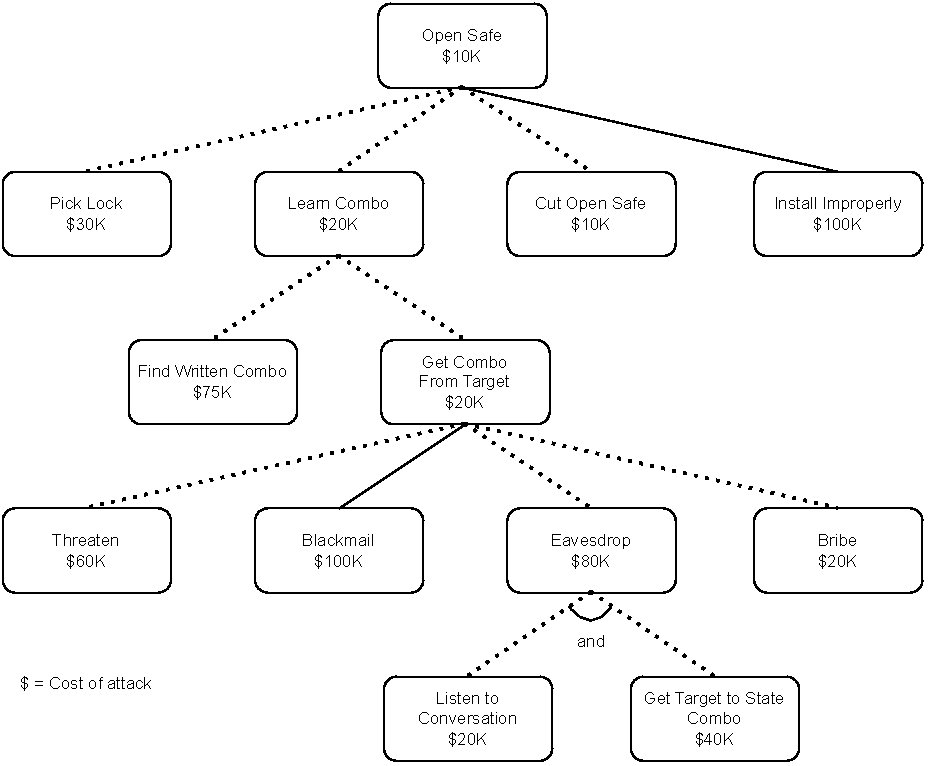
\includegraphics[width=0.8\linewidth]{figures/attack_graph.pdf}
  \caption[Illustration d'un graphe d'attaque décrivant un scénario de compromission d’un coffre-fort.]{Illustration d'un graphe d'attaque décrivant un scénario de compromission d’un coffre-fort. (adapté de \cite{schneier1999modeling})~: L’objectif racine \emph{Open Safe} est décomposé en quatre voies principales : \emph{Pick Lock} (\$30K), \emph{Learn Combo} (\$20K), \emph{Cut Open Safe} (\$10K) et \emph{Install Improperly} (\$100K). Par défaut, un nœud est de type \textsc{OU} (réaliser l’un des enfants suffit) ; lorsqu’un \emph{and} est indiqué, il s’agit d’un \textsc{ET} (tous les enfants sont requis). Les montants représentent des coûts estimés : pour un \textsc{OU}, le coût du parent est le \emph{minimum} des coûts enfants ; pour un \textsc{ET}, les coûts \emph{s’additionnent}.}
  \label{fig:attack_graphs}
\end{figure}

\noindent
\textbf{Arbres attaque-défense}~: \quad Les arbres attaque-défense~\cite{BKordy2010} (arbres \acparen{AD}) sont des modèles graphiques représentant les objectifs de l'attaquant et les contre-mesures du défenseur sous la forme d'une structure arborescente. Les arbres \acn{AD} fournissent une représentation plus abstraite du système et des objectifs des attaquants, tandis que les graphes d'attaque fournissent une représentation plus concrète des composants du système et de leurs relations. Un exemple d'arbre \acn{AD} est illustré en \autoref{fig:bank_attack_defense_tree}. La racine de l'arbre \acn{AD} représente l'objectif ultime des cyberattaquants. Les sous-nœuds associés aux branches représentent les différentes stratégies d'attaque que l'attaquant pourrait utiliser pour atteindre son objectif. Ils peuvent être accompagnés de contre-mesures préventives ou réactives du défenseur (pare-feu, systèmes de détection d'intrusion, plans d'intervention en cas d'incident, etc.).
Les arbres \acn{AD} permettent d'identifier les points faibles de la défense d'un système~\cite{BKordy2010}.

\begin{figure}[h]
  \centering
  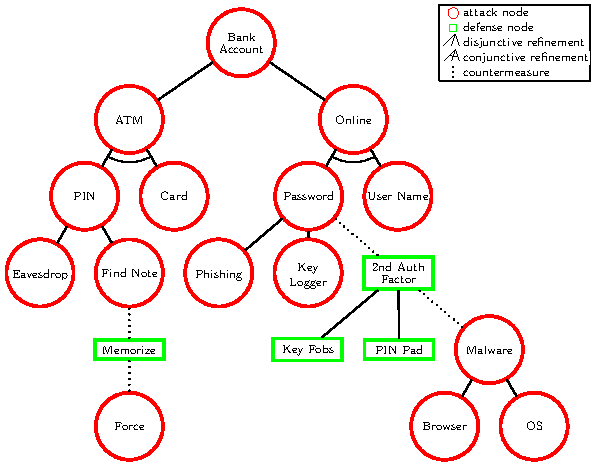
\includegraphics[width=\linewidth]{figures/adt.pdf}
  \caption[Illustration d'ADTree d'un scénario d'attaque sur un compte bancaire.]{Illustration d'ADTree décrivant un scénario d'attaque sur un compte bancaire. (tiré de \cite{BKordy2010})~: L'accès au compte peut être fait via un guichet automatique ou en ligne. Pour ce dernier cas, il est nécéssaire d'avoir un identifiant et un mot de passe obtenable par phishing ou un \textit{Key Logger}. Une contremesure à ces attaques est la double authentification construite avec une clé \textit{fob} ou un code pin.}
  \label{fig:bank_attack_defense_tree}
\end{figure}


\noindent
\textbf{Modélisation par réseaux de Petri}~: \quad Les réseaux de Petri pouvant être utilisés pour décrire des processus concurrents, certains travaux ont cherché à modéliser les attaquants et les défenseurs dans un système en réseau.
Les attaques extraites de bases de données peuvent être modélisées à l'aide de réseaux de Petri afin d'intégrer les cyberattaquants et les cyberdéfenseurs, leurs stratégies et le coût de leurs actions, comme dans ~\cite{MPetty2022}. Les réseaux de Petri se révèlent également utiles pour modéliser les attaques par injection de langage de requête structuré afin d'inclure les stratégies des joueurs~\cite{JBland2020}.
Ils sont utilisés comme cadre pour évaluer et comparer plusieurs modèles d'attaque.
Dans ~\cite{SYamaguchi2020}, le logiciel malveillant \textit{Mirai} a aussi été exprimé sous la forme d'un modèle formel avec des réseaux de Petri, permettant de simuler un combat entre un agent défenseur et \textit{Mirai}.

\

\noindent
\textbf{Modèles de jeu}~: \quad Certains travaux ont proposé de modéliser les interactions entre les attaquants et les défenseurs dans un réseau comme des joueurs dans un jeu, où chaque joueur dispose d'un ensemble d'actions qu'il peut effectuer.
Parmi les travaux notables, citons~: Panfili et al.~\cite{MPanfili2018}, où un jeu à somme générale multi-agents opposant un attaquant à un défenseur est utilisé pour trouver un compromis optimal entre les actions de prévention et les coûts~; Attiah et al.~\cite{AAttiah2018}, où un cadre théorique de jeu dynamique est proposé pour analyser les interactions entre l'attaquant et le défenseur comme un jeu de sécurité non coopératif~; et Xiaolin et al.~\cite{CXiaolin2008}, qui utilisent des modèles de processus de Markov pour évaluer les risques dans les systèmes en réseau.

\noindent
Certaines approches fondées sur la théorie des jeux s'inscrivent dans le cadre des \textquote{jeux stochastiques partiellement observables} (POSG) ou, plus précisément, dans celui des \textquote{processus de décision markoviens décentralisés partiellement observables} (Dec-POMDP). Les POSG et les Dec-POMDP sont tous deux des cadres de modélisation mathématique des problèmes de prise de décision dans lesquels des agents interagissent entre eux et dans un environnement stochastique~\cite{beynier2010}. Dans un POSG, un groupe d'agents interagit avec un environnement stochastique et partiellement observable. Chaque agent agit en fonction de ses propres observations et d'une politique locale. Les agents peuvent avoir des objectifs différents, car chaque agent a sa propre fonction de récompense et le jeu est généralement supposé être non coopératif~\cite{terry2020pettingzoo}. Dans un Dec-POMDP, plusieurs agents peuvent avoir une fonction de récompense commune et peuvent coordonner leurs actions pour atteindre un objectif commun, notamment en étant capables de communiquer~\cite{bernstein2013}.

\

\noindent
Afin de définir une modélisation, nous avons pris un cas d'utilisation tiré de l'AICA~\cite{theron_autonomous_2021}. Nous nous intéressons à la modélisation d'un environnement réseau composé de \textit{nœuds} sur lesquels des cyberattaquants et des cyberdéfenseurs \textit{agents} peuvent être déployés pour observer et agir. Ces nœuds peuvent être décrits par un ensemble de \textit{propriétés} liées aux processus, aux systèmes de fichiers, aux systèmes d'exploitation, à l'architecture matérielle, etc.
Les \textit{observations} et les \textit{actions} des agents sont conditionnées par leurs propres propriétés (y compris celles qu'ils connaissent) et par des incertitudes. Par exemple, la lecture d'un fichier donné ou le remappage de ports peut nécessiter un niveau de privilège élevé~; ou la réception de données provenant d'un capteur physique n'est pas garantie à tout moment.
Chaque agent qui applique des actions modifie les propriétés d'un ou plusieurs nœuds. Cela modifie l'état de l'environnement, rapprochant ou éloignant les agents de leur objectif.
Les principales caractéristiques de cette description englobent des notions telles que l'incertitude dans les observations, les conditions dans les actions pour la transition d'état et les métriques que nous considérons comme exprimées dans une modélisation Dec-POMDP.
%\after{Ceci vise à répondre au besoin d'un modèle formel d'agents attaquants et défenseurs englobant divers contextes d'application.}



\subsection{Les \textit{World Models} pour automatiser la modélisation en simulation}

En \acn{RL}, et en particulier en contexte d'observabilité partielle, les \textbf{modèles du monde}~\cite{ha2018recurrent, hafner2020dream} visent à apprendre des modèles internes approximant à la fois la dynamique de la fonction de transition et d'observation conjointement. Les \textit{World Models} permettent aux agents d'effectuer de la planification, d'améliorer l'efficacité échantillonnale, et de faciliter l'exploration sûre en permettant à l'agent de simuler des scénarios futurs. Cette approche appartient au paradigme du \acn{MBRL}~\cite{moerland2020model}, et se révèle particulièrement utile pour construire automatiquement des modèles de simulation à haute fidélité même en l'absence de représentation explicite de l'environnement.

Formellement, à chaque pas de temps $t$, on note $\omega_t \in \Omega$ l'observation courante, $a_t \in A$ l'action réalisée, et $\tilde{h}_{t-1} \in \mathcal{H}$ l'état caché récurrent résumant l'historique d'interaction jusqu'à $t-1$. Étant donné que les observations sont généralement de grande dimension (par exemple, des images ou des vecteurs d'état complexes), un encodeur $Enc: \Omega \rightarrow Z$ est appliqué pour projeter les observations dans un espace latent compact $Z$, avec $z_t = Enc(\omega_t)$, où $\dim(Z) \ll \dim(\Omega)$.

La structure temporelle principale est modélisée à l'aide d'un \textbf{Modèle Dynamique Latent Récurrent (\acparen{RLDM})}~\cite{hafner2020dream} $\mathcal{T}^{z} = f(g(h_{t-1}, z_t, a_t))$, qui prédit le prochain état latent $z_{t+1}$ en mettant à jour l'état récurrent via $f$ et en appliquant une dynamique latente via $g$~:
\[
  h_t = f(h_{t-1}, z_t, a_t), \quad z_{t+1} = g(h_t)
\]
où $f(\cdot)$ correspond typiquement à un réseau de neurones récurrent (par exemple un \acparen{LSTM}~\cite{hochreiter1997long}) appliqué à la concaténation de $h_{t-1}$, $z_t$ et $a_t$, et $g(\cdot)$ est une fonction (souvent implémentée par un \acparen{MLP}) mappant l'état récurrent vers la représentation latente de la prochaine observation.

L'état latent prédit est ensuite décodé par $Dec: Z \rightarrow \Omega$ pour produire l'observation prédite $\hat{\omega}_{t+1} = Dec(z_{t+1})$. L'ensemble du modèle est entraîné conjointement pour minimiser à la fois la \emph{perte de reconstruction} $\|\omega_{t+1} - \hat{\omega}_{t+1}\|$ dans l'espace d'observation, et éventuellement une \emph{perte de prédiction latente} pour stabiliser l'apprentissage de la dynamique latente.

L'état caché récurrent $\tilde{h}_t$ joue le rôle d'un résumé compact de l'historique complet d'interaction jusqu'au temps $t$, évitant ainsi d'avoir à stocker explicitement de longues séquences observation-action.

Par souci de concision, nous définissons la composition complète qui associe directement observation courante, action et état récurrent à l'observation prédite suivante sous la forme du \textbf{Modèle de Prédiction d'Observation}~:
\[
  \mathcal{T}(h_{t-1}, \omega_t, a_t)~:= Dec(g(f(h_{t-1}, Enc(\omega_t), a_t))) = \hat{\omega}_{t+1}.
\]

\subsection{Défis et perspectives}

Plusieurs limites subsistent dans l'utilisation des \textit{World Models} pour les \acn{SMA}~:
\begin{itemize}
  \item \textbf{Apprentissage à partir de données partielles ou bruitées}, typiques des environnements partiellement observables~;
  \item \textbf{Généralisation limitée} à des situations non vues ou à de nouveaux agents~;
  \item \textbf{Intégration difficile} avec les algorithmes \acn{MARL} standards, notamment pour la planification à long terme ou le guidage explicite.
\end{itemize}

D'autre part, appliquer les \textit{World Models} dans un cadre multi-agent soulève des défis supplémentaires~:
\begin{itemize}
  \item \textbf{Représentation conjointe}~: il faut encoder plusieurs observations locales (souvent hétérogènes) dans un espace commun latent~;
  \item \textbf{Coordination implicite}~: le modèle doit capturer les effets d'interaction entre agents, y compris lorsque les comportements sont dépendants~;
  \item \textbf{Complexité combinatoire}~: le nombre d'agents et de combinaisons d'actions croît rapidement, rendant l'apprentissage difficile.
\end{itemize}

Ces défis ouvrent la voie à des approches hybrides où les \textit{World Models} ne servent pas uniquement à l'apprentissage de dynamiques internes orientées pour l'apprentissage de l'agent, mais aussi à la modélisation d'environnements simulés contraints et guidés, comme proposé dans notre méthode.


\chapter{Les verrous d'une méthode de conception}
\label{chap:verrous}

\noindent
Le chapitre précédent a introduit les concepts fondamentaux nécessaires à la compréhension de notre démarche, en s'appuyant sur trois piliers théoriques~: l'organisation explicite des \acn{SMA} à travers des modèles comme \textit{$\mathcal{M}OISE^+$}, \acn{MARL}, et les techniques de modélisation d'environnement via les \textit{World Models} notamment. Ces notions constituent l'ossature sur laquelle repose notre méthode de conception.

Toutefois, ces cadres théoriques, pris isolément, ne permettent pas de répondre aux exigences posées par la thèse dans le \autoref{chap:verrous}. En particulier, la conception automatique d'un \acn{SMA} adapté à un environnement cible reste limitée par plusieurs obstacles théoriques ou technologiques, que nous identifions ici comme des \textit{verrous scientifiques}.

Ce chapitre a pour objectif d'analyser, pour chacune des hypothèses H1 à H4 formulées précédemment, l'état de l'art pertinent, les manques ou limites existants, ainsi que les verrous associés. Il s'agit ainsi d'établir une cartographie critique des défis que notre méthode devra relever, tout en préparant les fondations conceptuelles de la \autoref{part:methode}, où nous présentons notre réponse méthodologique sous la forme de la méthode \acn{MAMAD}.


\section{Les Worlds Models pour simuler des environnement multi-agents}

\noindent
Les travaux présentés dans le \autoref{chap:concepts} ont montré l'intérêt de disposer d'un environnement simulé pour entraîner des agents de manière sûre, rapide et contrôlée. Dans cette perspective, les \textit{World Models} constituent une approche prometteuse, permettant d'apprendre une dynamique approximative de l'environnement à partir de données collectées. Ces modèles sont largement utilisés en apprentissage par renforcement, notamment dans des contextes mono-agent, mais restent sous-explorés en environnement multi-agent complexe.

\medskip

\noindent
La littérature récente montre un regain d'intérêt pour l'automatisation de la conception de \acn{SMA}, notamment via l'ingénierie dirigée par les modèles, les frameworks organisationnels paramétrables, ou encore les générateurs de code à partir de spécifications. Des travaux comme INGENIAS~\cite{Pavon2003}, KB-ORG~\cite{Sims2008} ou AutoGenesisAgent~\cite{harper2024autogenesisagent} visent à automatiser la génération d'architectures agents à partir de modèles symboliques. Néanmoins, ces approches supposent en général un environnement connu, structuré, voire entièrement spécifié a priori.

\noindent
Dans le domaine de l'apprentissage, des travaux récents en cybersécurité~\cite{hammar2023scalable} ont exploré la génération automatique de scénarios pour entraîner des agents en simulation. Ces environnements, bien que plus dynamiques, sont encore conçus manuellement ou via des générateurs à base de règles, et ne s'adaptent pas aux interactions des agents. À ce jour, aucun pipeline complet ne relie la collecte de données dans un environnement réel à l'entraînement de politiques multi-agents via un modèle simulé appris de manière autonome.

\medskip

\noindent
Le cadre des World Models~\cite{Ha2018} propose une solution intéressante à ce besoin. En apprenant une représentation latente compressée de l'environnement et sa dynamique, il devient possible de simuler des trajectoires cohérentes pour entraîner des politiques sans interaction réelle. Toutefois, ces approches ont été principalement développées pour des environnements mono-agents à observation complète.

\noindent
Appliquer les \textit{World Models} à des environnements multi-agents soulève plusieurs défis~:
\begin{itemize}
  \item \textbf{Représentation conjointe}~: comment encoder et combiner des observations partielles issues de plusieurs agents hétérogènes~;
  \item \textbf{Dynamique coordonnée}~: comment apprendre une transition qui tient compte des effets d'interaction ou de coopération~;
  \item \textbf{Évolutivité}~: comment maintenir la qualité de la simulation lorsque le nombre d'agents et d'actions augmente.
\end{itemize}

\noindent
À notre connaissance, aucune approche ne propose actuellement un \textit{World Model} multi-agent générique capable de simuler des environnements partiellement observables avec des interactions complexes entre agents. Cela constitue un verrou méthodologique majeur à l'automatisation de la conception de \acn{SMA}~: sans modèle simulé réaliste, il est difficile de guider ou d'évaluer l'apprentissage des politiques à grande échelle.

\medskip

\noindent
\textbf{Hypothèse H2~:} il est possible d'apprendre automatiquement un modèle simulé multi-agent (World Model) à partir de trajectoires collectées dans un environnement cible, en combinant des représentations latentes et des prédictions conjointes adaptées à l'apprentissage multi-agent.


\section{L'intégration de contraintes/guidages organisationnelles dans le processus MARL}

\noindent
Le \acn{MARL}, tel que présenté dans le \autoref{chap:concepts}, permet aux agents de développer de manière autonome des politiques coopératives dans des environnements complexes et dynamiques. Toutefois, la nature exploratoire du \acn{MARL} rend difficile le contrôle précis des comportements émergents, en particulier lorsque des exigences critiques de sûreté, de coordination ou de structure doivent être respectées.

\medskip

\noindent
Les travaux en \textit{Safe Reinforcement Learning} ont cherché à intégrer des contraintes dans le processus d'apprentissage afin d'éviter certains comportements indésirables. Par exemple, \acn{CPO}~\cite{achiam2017constrained} garantit que la politique reste proche d'un ensemble d'actions autorisées, tandis que \textit{Deep Constrained Q-Learning}~\cite{kalweit2020deep} applique des contraintes explicites sur la mise à jour des valeurs Q. D'autres approches introduisent des mécanismes de \textit{shielding}, \textit{reward shaping} ou encore l'intégration de retours humains (cf.~\cite{zhou2025mentor}). Ces travaux montrent qu'il est possible d'influencer l'apprentissage en encadrant l'espace des politiques, tout en maintenant une capacité d'adaptation.

\noindent
Cependant, la majorité de ces méthodes opèrent à un niveau \textit{comportemental} local~: elles imposent des règles sur les actions possibles, ou ajustent la récompense pour favoriser certaines trajectoires. Très peu de travaux intègrent des contraintes \textit{organisationnelles} symboliques, c'est-à-dire des spécifications abstraites sur les rôles, missions ou interactions attendues entre agents.

\medskip

\noindent
La littérature sur le \acn{MARL} s'est principalement concentrée sur l'optimisation de la coopération entre agents dans des environnements incertains et partiellement observables~\cite{Zhang2021, Papoudakis2021}. Toutefois, les approches classiques négligent généralement l'incorporation de contraintes symboliques ou organisationnelles dans le processus d'apprentissage. Les agents apprennent par essais-erreurs sans garantie que leurs comportements émergents respecteront des exigences de conception critiques, comme des règles de sûreté, le respect des rôles, ou des hiérarchies d'équipe.

\noindent
Plusieurs travaux récents ont tenté de combler cette lacune via des techniques d'apprentissage par renforcement sensibles aux contraintes. \textit{Constraint-Guided Reinforcement Learning}~\cite{spieker2021constraint} intègre des modèles de contraintes explicites dans l'interaction agent-environnement, permettant d'apprendre des politiques respectant des bornes comportementales prédéfinies. \textit{Deep Constrained Q-Learning}~\cite{kalweit2020deep} impose des contraintes à court et moyen terme dans la mise à jour des valeurs Q, assurant ainsi le respect de critères de performance et de sécurité. L'approche \acn{CPO}~\cite{achiam2017constrained} offre des garanties théoriques de satisfaction des contraintes durant la recherche de politiques, et \textit{MENTOR}~\cite{zhou2025mentor} guide les agents dans un cadre hiérarchique à l'aide de retours humains et de sous-objectifs dynamiquement contraints. Enfin, l'apprentissage contraint sans fonction de récompense explicite~\cite{miryoosefi2022} optimise directement la satisfaction de contraintes en contournant l'ingénierie de récompenses.

\medskip

\noindent
Si ces approches renforcent le contrôle des politiques apprises, elles restent limitées à un niveau local ou comportemental et n'intègrent pas des modèles de conception symboliques tels que ceux développés en ingénierie des \acn{SMA}.

\medskip

\noindent
Les modèles issus de l'ingénierie des \acn{SMA}, comme \textit{$\mathcal{M}OISE^+$}~\cite{hubner2002moise}, proposent au contraire une structuration explicite du système via des rôles, des missions à accomplir, et des groupes formés dynamiquement. À notre connaissance, aucune approche ne permet de guider ou contraindre les agents à s'aligner sur des comportements d'agents évoluant dans une organisation structurée et fonctionnelle telle que proposée dans $\mathcal{M}OISE^+$.


%ttt

\medskip

\noindent
Ainsi, un verrou fondamental demeure~: il n'existe pas de méthode permettant de structurer et de guider l'apprentissage \acn{MARL} à partir de spécifications organisationnelles riches, telles que celles proposées par $\mathcal{M}OISE^+$, tout en assurant un compromis entre autonomie d'apprentissage et respect de contraintes. Or, dans des domaines critiques (cyberdéfense, secours, coordination robotique), ce besoin est central.

\medskip

\noindent
\textbf{Hypothèse H3~:} il est possible de contraindre ou guider l'apprentissage multi-agent en intégrant des spécifications organisationnelles (rôles, missions, groupes) sous forme de contraintes explicites, afin de produire des politiques sûres, coordonnées et explicables, sans restreindre excessivement la capacité d'apprentissage des agents.


\section{L'extraction automatisée des spécifications organisationnelles émergentes}

Alors que la tradition \acn{AOSE} garantit l'explicabilité à travers des artefacts de conception structurés (tels que des protocoles, des rôles, des missions ou des objectifs), ces éléments symboliques sont généralement perdus dans les approches classiques du \acn{MARL}. Les politiques apprises sont souvent représentées sous la forme de réseaux de neurones opaques, rendant difficile l'évaluation de la conformité des comportements des agents avec l'intention de conception initiale ou les principes organisationnels. Bien que l'explicabilité en \acn{MARL} ait suscité un intérêt croissant, la majorité des travaux existants se concentrent sur le comportement individuel des agents ou les mécanismes internes des politiques, sans aborder leur alignement collectif ou organisationnel.

Un nombre croissant de recherches cherche à améliorer l'interprétabilité via la conception de modèles ou l'analyse post-hoc. Zabounidis et al.~\cite{zabounidis2023concept} intègrent des concepts interprétables dans la boucle d'apprentissage, en forçant les agents à prédire des concepts compréhensibles par un humain avant d'agir. Cela favorise la transparence et permet des corrections par des experts. Iturria-Rivera et al.~\cite{iturria2024explainable} utilisent la décomposition de la récompense dans les fonctions de valeur factorisées (par exemple VDN, QMIX) pour exposer la contriobjectifion de chaque composante aux décisions de l'agent. Liu et al.~\cite{liu2025} proposent MIXRTs, une architecture hybride combinant réseaux neuronaux récurrents et arbres de décision pour l'apprentissage de politiques interprétables. D'autres efforts comme ceux de Poupart et al.~\cite{poupart2025perspectives} introduisent des méthodes post-hoc telles que la rétropropagation de la pertinence (relevance backpropagation) ou le patching d'activations. Li et al.~\cite{li2025from} emploient des approximations basées sur la valeur de Shapley pour transformer des politiques de type deep \acn{RL} en structures interprétables.

Cependant, ces approches restent principalement limitées à des analyses locales ou centrées sur un seul agent. Elles ne permettent pas d'interpréter le comportement collectif d'un \acn{SMA} ni de relier ces dynamiques à des structures organisationnelles symboliques. Très peu d'études abordent explicitement la possibilité d'inférer des rôles, objectifs ou structures émergentes à partir de trajectoires observées.

Certains travaux connexes offrent néanmoins des pistes intéressantes. Berenji et Vengerov~\cite{berenji2000learning} modélisent les dépendances entre agents dans des missions de drones afin d'améliorer leur coordination, et Yusuf et Baber~\cite{yusuf2020inferential} proposent un raisonnement bayésien pour soutenir une coordination dynamique. Bien que ces contriobjectifions soulignent l'intérêt d'une modélisation symbolique à partir de comportements, elles ne fournissent pas de mécanismes pour inférer explicitement des rôles ou objectifs organisationnels à partir des trajectoires. De leur côté, Serrino et al.~\cite{serrino2019finding} analysent les interactions sociales pour identifier des rôles émergents, mais leur approche reste centrée sur des dynamiques sociales informelles sans formalisation organisationnelle.

En résumé, aucune méthode existante ne permet actuellement d'extraire automatiquement des spécifications organisationnelles (telles que des structures de rôles, des missions ou des objectifs collectifs) à partir de trajectoires d'agents entraînés. Or, une telle capacité permettrait de combler le fossé entre les approches symboliques prescriptives de l'\acn{AOSE} et les approches apprenantes fondées sur l'émergence. Elle offrirait un cadre pour évaluer l'organisation implicite d'un \acn{SMA}, identifier des écarts avec un modèle attendu, et potentiellement réinjecter ces connaissances dans une boucle de conception organisationnelle itérative. Cette hypothèse ouvre la voie à une nouvelle génération de méthodes de diagnostic, de rétro-ingénierie et d'adaptation des \acn{SMA} entraînés par apprentissage.

\medskip

\noindent
\textbf{Hypothèse H4~:} il est possible d'inférer automatiquement des spécifications organisationnelles émergentes à partir des trajectoires d'agents entraînés, en combinant des techniques d'analyse symbolique, de clustering comportemental et de projection organisationnelle, afin d'évaluer et d'adapter l'organisation d'un \acn{SMA} de manière itérative.


\section{Un cadre Markovien pour formaliser le problème de conception et sa résolution en MARL}

\noindent
La conception d'un \acn{SMA} implique généralement de définir des rôles, des interactions et des règles de coordination dans un environnement donné. Traditionnellement, cette activité repose sur une modélisation symbolique, où les concepteurs spécifient manuellement les comportements et les structures attendus. À l'inverse, les approches fondées sur l'apprentissage, notamment le \acn{MARL}, cherchent à découvrir ces comportements de manière automatique à partir d'expériences. Il devient alors essentiel de disposer d'un cadre formel permettant de représenter le problème de conception lui-même comme un problème de décision, résoluble par apprentissage.

\medskip

\noindent
Les travaux en \acn{MARL} se basent généralement sur des modèles Markoviens multi-agents, tels que les \acn{Dec-MDP} ou les \acn{Dec-POMDP}. Dans un \acn{Dec-POMDP}, chaque agent dispose d'observations partielles, d'une politique locale, et d'une fonction de récompense partagée ou individuelle. Ce formalisme permet de représenter des dynamiques complexes, distribuées et incertaines, tout en tenant compte de la coordination nécessaire entre agents.

\noindent
Cependant, dans la majorité des cas, ces modèles sont utilisés pour représenter des problèmes d'exécution (ex.~: résolution de tâches) plutôt que des problèmes de conception. Le lien entre spécifications organisationnelles ($\mathcal{M}OISE^+$, rôles, missions) et les composantes du \acn{Dec-POMDP} n'est généralement pas formalisé. De plus, ces modèles ne permettent pas directement d'imposer des contraintes symboliques sur les politiques ou les trajectoires.

\medskip

\noindent
Pour pallier cette limite, plusieurs extensions des \acn{MDP}s ont été proposées~:
\begin{itemize}
  \item les \textit{Constrained \acn{MDP}} (CMDP), où certaines contraintes (coût, sécurité) doivent être respectées au cours de l'exécution~;
  \item les \textit{Constrained \acn{Dec-POMDP}}, qui introduisent des contraintes globales ou locales sur les politiques des agents~;
  \item les formulations basées sur des \textit{specifications logiques} pour encadrer l'espace des politiques admissibles.
\end{itemize}

\noindent
Ces modèles constituent des bases intéressantes, mais restent rarement utilisés pour formaliser le processus même de \textit{conception} d'un \acn{SMA}. En effet, ils supposent généralement que la dynamique de l'environnement est connue, que l'espace d'état est spécifié, et que les contraintes sont codées à bas niveau. Il manque donc un cadre unifié permettant de représenter~:
\begin{itemize}
  \item les dynamiques simulées de l'environnement (World Model)~;
  \item les contraintes organisationnelles ($\mathcal{M}OISE^+$)~;
  \item et la recherche de politiques collectives compatibles avec ces éléments.
\end{itemize}

\medskip

\noindent
Nous proposons d'enrichir le \acn{Dec-POMDP} en y injectant deux structures complémentaires~:
\begin{enumerate}
  \item une fonction d'environnement $\mathcal{T}$, apprise à partir de données (World Model)~;
  \item un ensemble de contraintes organisationnelles symboliques, représentées sous forme de relations $(h, o) \mapsto A_{autorisé}$ ou de fonctions de récompense de trajectoire.
\end{enumerate}

\noindent
L'idée est de voir la conception d'un \acn{SMA} comme un \textit{problème d'optimisation sous contraintes}, où les politiques sont apprises pour maximiser une récompense tout en respectant des contraintes structurelles, organisationnelles ou comportementales. Cette formalisation ouvre la voie à un apprentissage dirigé et sécurisé des comportements.

\medskip

\noindent
\textbf{Hypothèse H1~:} il est possible de formaliser le problème de conception d'un \acn{SMA} comme un problème d'optimisation dans un cadre \acn{Dec-POMDP} enrichi, en y intégrant à la fois un modèle simulé de l'environnement (World Model) et des contraintes organisationnelles dérivées d'un modèle comme $\mathcal{M}OISE^+$.

\section*{Synthèse des verrous identifiés}

\noindent
Ce chapitre a permis d'établir un lien entre les hypothèses de recherche formulées en \autoref{part:contexte}, l'état de l'art dans les domaines concernés, et les verrous scientifiques empêchant aujourd'hui une conception automatisée, sûre et explicable des systèmes multi-agents.

\medskip

\noindent
Le \autoref{tab:verrous_hypotheses} synthétise cette analyse. Il met en évidence que, malgré des avancées importantes dans des domaines comme le \acn{MARL}, la simulation via World Models, l'apprentissage contraint, ou l'explicabilité, aucun cadre existant ne permet aujourd'hui de traiter conjointement~:
\begin{itemize}
  \item la modélisation dynamique d'un environnement inconnu (H2)~;
  \item l'apprentissage multi-agent sous contraintes structurelles (H3)~;
  \item l'analyse organisationnelle des comportements appris (H4)~;
  \item et la formalisation complète de ce processus dans un cadre décisionnel résoluble (H1).
\end{itemize}

\noindent
Ces lacunes justifient la nécessité d'une approche intégrée, qui articule apprentissage, organisation et analyse dans une boucle de conception fermée. Les hypothèses H1 à H4 révèlent ainsi quatre besoins méthodologiques complémentaires, qui seront pris en charge dans notre proposition.

\medskip

\noindent
La partie suivante introduit la méthode \textbf{\acn{MAMAD}} (\acparen{SMA}), développée précisément pour répondre à ces besoins. Cette méthode repose sur une formalisation unifiée du processus de conception comme un problème d'optimisation organisationnelle sous contraintes, résolu par apprentissage, simulé via un World Model, et analysé en retour pour guider les itérations futures.


\begin{table}[H]
  \centering
  \caption{Synthèse des travaux prometteurs, verrous, limites et besoins méthodologiques par hypothèse}
  \label{tab:synthese_hypotheses}
  \renewcommand{\arraystretch}{1.2}
  {%
    \footnotesize
    \begin{tabularx}{\textwidth}{cXXXX}
      \hline
      \textbf{Hyp.}
       & \textbf{Travaux prometteurs}
       & \textbf{Verrous principaux}
       & \textbf{Limites des travaux existants}
       & \textbf{Besoins méthodologiques}                                                                                                                                                                      \\
      \hline

      \textbf{H-MOD}
       & Dec-POMDP comme cadre adaptable ; World Models pour la modélisation automatique
       & Lourdeur de la modélisation manuelle ; absence de bibliothèques spécialisées cyber ; extension multi-agent des World Models non résolue
       & World Models limités au mono-agent ou à des contextes simples ; peu d'approches exploitant des observations distribuées ; modèles markoviens trop simples pour aider à la modélisation manuelle
       & Apprendre un World Model multi-agent structuré autour de représentations latentes ; proposer un modèle markovien utilisable pour modéliser un environnement de cyberdéfense                           \\
      \hdashline

      \textbf{H-TRN}
       & Safe RL (CPO, DCQL) ; Constraint-Guided RL ; intégration potentielle de modèles organisationnels (MOISE+)
       & Faible expressivité organisationnelle des méthodes existantes ; absence de cadre unifié entre organisation symbolique et MARL ; manque de garanties globales
       & Constrained RL ne prend pas en compte les structures organisationnelles ; intégration de spécifications symboliques limitée à l'exécution
       & Introduire des contraintes symboliques dans le processus MARL pour guider l'apprentissage et filtrer les actions                                                                                      \\
      \hdashline

      \textbf{H-ANL}
       & MAVIPER et modèles interprétables ; clustering de trajectoires pour inférence de rôles ; ROMA
       & Absence de lien avec modèles symboliques ; manque d'automatisation ; pas de cadre d'évaluation de l'explicabilité organisationnelle
       & Explicabilité surtout locale (niveau agent/action) ; peu de travaux inférant des rôles, missions ou objectifs collectifs
       & Inférer automatiquement rôles, missions et objectifs à partir de trajectoires ; proposer un cadre théorique pour l'explicabilité organisationnelle                                                    \\
      \hdashline

      \textbf{H-TRF}
       & Domain adaptation / Sim2Real ; Robust RL ; Online calibration (PILCO)
       & Approches partielles (transfert ou recalibrage, mais pas les deux) ; absence de cadre intégré de jumeau numérique adaptatif et de mise à jour conjointe des politiques
       & Domain adaptation et sim2real se concentrent sur le transfert initial sans recalibrage dynamique ; robust RL ne met pas à jour le modèle simulé ; calibration en ligne sans adaptation des politiques
       & Développer un framework unificateur de jumeau numérique couplant mise à jour continue du modèle simulé et adaptation conjointe des politiques multi-agents                                            \\
      \hline
    \end{tabularx}
  }
\end{table}


\clearpage
\thispagestyle{empty}
\null
\newpage

\chapter*{Conclusion}
\addcontentsline{toc}{chapter}{\textbf{Conclusion}}

\noindent
Cette deuxième partie a posé les fondations théoriques et critiques nécessaires à l'élaboration de notre méthode de conception. En s'appuyant sur les enjeux identifiés dans la \autoref{part:contexte}, elle a permis de clarifier les concepts mobilisés, d'identifier les manques persistants dans la littérature, et de formuler les verrous qui justifient la nécessité d'une nouvelle approche.

\medskip

\noindent
Le \autoref{chap:concepts} a introduit les trois piliers conceptuels sur lesquels s'appuie notre démarche~: (1) les modèles organisationnels, en particulier \textit{$\mathcal{M}OISE^+$}, qui offrent une structuration explicite du \acn{SMA}~; (2) Le \acn{MARL}, qui permet une acquisition autonome de politiques dans des environnements complexes~; et (3) les \textit{World Models}, qui fournissent un moyen de simuler un environnement à partir de données, ouvrant la voie à une exploration sécurisée et accélérée.

\noindent
Le \autoref{chap:verrous} a prolongé cette analyse en examinant les limites de l'état de l'art face aux exigences soulevées par notre question. Chaque hypothèse de recherche (H1 à H4) a été replacée dans son contexte scientifique, discutée à la lumière des travaux existants, et reliée à un verrou spécifique~:
\begin{itemize}
  \item la difficulté à représenter le problème de conception dans un cadre décisionnel formel (H1)~;
  \item l'absence de \textit{World Models} adaptés au contexte multi-agent (H2)~;
  \item le manque d'intégration de contraintes organisationnelles dans l'apprentissage (H3)~;
  \item l'impossibilité d'analyser les comportements appris à l'échelle organisationnelle (H4).
\end{itemize}

\medskip

\noindent
Ces constats convergent vers un besoin commun~: celui d'une méthode unifiée, capable d'orchestrer l'ensemble du processus de conception (de la modélisation de l'environnement à l'analyse des comportements) en intégrant apprentissage et organisation dans une boucle cohérente. C'est précisément l'objectif de la méthode \acn{MAMAD}, que nous introduisons dans la partie suivante.

\noindent
La \autoref{part:methode} présente cette méthode en détail. Elle repose sur une formalisation du problème de conception comme un \acn{Dec-POMDP} contraint enrichi par des structures organisationnelles. \acn{MAMAD} articule quatre étapes principales (modélisation, apprentissage, analyse et transfert) pour automatiser, structurer et affiner la conception des \acn{SMA} dans des environnements dynamiques et incertains.
